Die Aufgabenstellung habe ich in foglende Teilaufgaben eingeteilt:
\begin{enumerate}
	\item Finden der mögichen Hautschuppen
	\item Filtern, welche der Hautschuppen tatsächlich zu einem Rhinozelfanten gehören
	\item Einfärben des gesamten Rhinozelfanten
\end{enumerate}

Eine Hautschuppe haben wir als Pixel definiert, das mehr als 2 gleichfarbige Nachbarfelder hat. Nachbarfelder sind alle direkt und diagonal anliegenden Pixel.

Diese Hautschuppenmenge enthält allerdings noch einige vermeintliche Hautschuppen, die zu keinem Rhinozoelefanten gehören. Beispielsweise werden oft Pixel im Himmel als Hautschuppe erkannt, da nur wenige Blautöne vorliegen. Diese False Positives müssen für ein besseres Ausgabebild herausgefiltert werden.

Dazu habe ich zuerst das Problem vereinfacht: Anstatt dies direkt auf dem bunten Bild durchzuführen, wird ein Schwarz-Weiß-Bild erstellt. In diesem Bild sind schwarze Pixel mögliche Hautschuppen, weiße Felder sind auf keinen Fall Hautschuppen. Dieses Zwischenbild wird Ihnen in der GUI angezeigt.

Auf dieses werden folgende Filter angewandt, um zu bestimmen welche möglichen Hautschuppen tatsächlich Teil eines Rhinozelfanten sind.

\begin{description}
	\item[Linienfilter] Zuerst wird nach ausreichend großen durchgehenden Linien gesucht: Einzelne Hautschuppen können schließlich keine Rhinozelfanten sein. Ich habe festgelegt, dass ein Rhinozelfant an seiner dicksten Stelle 4\% der Gesamtbreite des Bildes haben muss. Dies überschreiten alle Rhinozelfanten in den Beispielen deutlich. Kleinere Werte würden die Laufzeit erheblich verlängern, da mehr mögliche Rhinozelfanten an die nachfolgenden Filter weitergegeben werden würden. Größere Filter würden dementsprechend den Programmablauf beschleunigen, es könnten jedoch Rhinozelfanten übersehen werden. Alle Linien, die dieses Kriterium erfüllen, werden an den nächsten Filter weitergegeben.
	\item[Rechteckfilter] In den Bauch eines Rhinzelfanten lässt sich ein Rechteck zeichnen. In diesem Schritt wird überprüft, ob sich mit der soeben gefundenen Linie als obere Kante ein Rechteck höher als 1,25\% der Gesamthöhe des Bildes zeichnen lässt. Alle Rechtecke, die dieses Kriterium erfüllen, werden an den nächsten Filter weitergegeben.
	\item[Anatomiefilter] Zuletzt wird überprüft, ob sich das Umfeld des Rechteckes mit der Anatomie eines Rhinozelfanten deckt. Dazu wird überprüft, ob sich an das Rechteck Beine anzeichnen lassen. Auf den Rüssel wird nicht eingegangen, da seine Position stark variiert und die drei vorher genannten Filter keine False Positives gefunden haben.
\end{description}

Wenn von einer Stelle ausgehend all diese Kriterien zutreffen, sind alle zusammenhängenden Hautschuppen ein Rhinozelfant. Zwei Hautschuppen hängen zusammen, wenn sie benachbart sind.

\clearpage
Beispiel: \vspace{3em}
\begin{figure}[!ht]
	\centering
	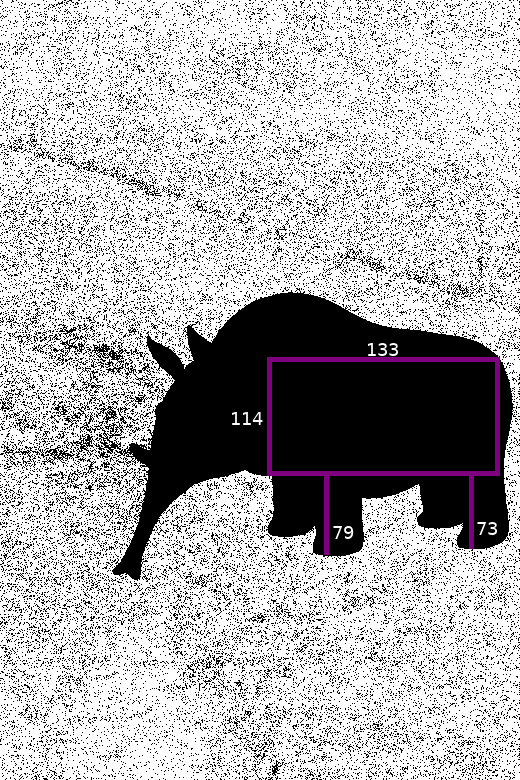
\includegraphics[width=0.7\textwidth]{SkizzeIdee4}
	\caption {Bsp. 4. mit eingezeichneten Skelett}
	Um den Filtereffekt zu verdeutlichen, wurde jedes Pixel mit mehr als einem gleichfarbigen Nachbar markiert.
\end{figure}